\setlength{\columnsep}{3pt}
\begin{flushleft}
\bigskip

\begin{itemize}
	\item \textbf{Systemd is the first process} that starts on system boot up.
	\item Systemd is a system and service manager for Linux OS.
	\item Systemd introduces the concept of systemd units. 
	\item Units are represented as unit configuration files located under:
	\begin{itemize}
		\item /usr/lib/systemd/system/
		\item /run/systemd/system/
		\item /etc/systemd/system/
	\end{itemize}
	\bigskip
	List all systemd units:
	\bigskip
	\begin{tcolorbox}[breakable,notitle,boxrule=0pt,colback=pink,colframe=pink]
		\color{black}
		\fontdimen2\font=1em
		Syntax: systemctl -t help
		\newline
		Syntax: systemctl list-unit-files
		\fontdimen2\font=4pt
	\end{tcolorbox}

	\begin{figure}[h!]
		\centering
		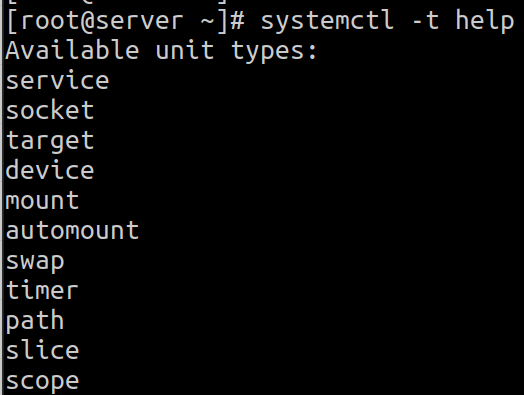
\includegraphics[scale=.5]{content/chapter17/images/systemd.png}
		\caption{Sample output}
		\label{fig:cpu256}
	\end{figure}
	
\newpage
	
	\paragraph{Managing services \& targets with systemd}

	\textbf{systemctl}: Controls the systemd system and services.

	\bigskip
	\begin{tcolorbox}[breakable,notitle,boxrule=0pt,colback=pink,colframe=pink]
		\color{black}
		\fontdimen2\font=1em
		Syntax: systemctl [options] [arguments]
		\fontdimen2\font=4pt
	\end{tcolorbox}
	\bigskip
	
	Options with \textbf{systemctl} command:
	\begin{itemize}
		\item \textbf{start}: Start a service/daemon.	 
		\bigskip
		\begin{tcolorbox}[breakable,notitle,boxrule=0pt,colback=pink,colframe=pink]
			\color{black}
			\fontdimen2\font=1em
			Syntax: systemctl start [service-name]
			\fontdimen2\font=4pt
		\end{tcolorbox}
		
		\bigskip
		\bigskip

		\item \textbf{status}: Display status of a service/daemon.	 
		\bigskip
		\begin{tcolorbox}[breakable,notitle,boxrule=0pt,colback=pink,colframe=pink]
			\color{black}
			\fontdimen2\font=1em
			Syntax: systemctl status [service-name]
			\fontdimen2\font=4pt
		\end{tcolorbox}
		
		Eg:
		\begin{figure}[h!]
			\centering
			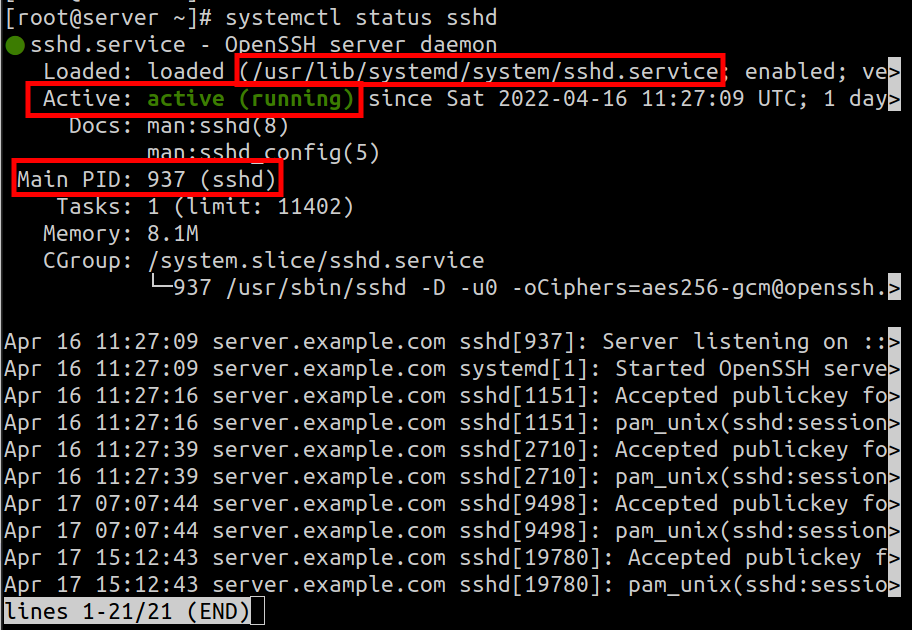
\includegraphics[scale=.3]{content/chapter17/images/status.png}
			\caption{Sample output}
			\label{fig:free_h_s}
		\end{figure}
		
		\item \textbf{stop}: Stop a service/daemon.	 
		\bigskip
		\begin{tcolorbox}[breakable,notitle,boxrule=0pt,colback=pink,colframe=pink]
			\color{black}
			\fontdimen2\font=1em
			Syntax: systemctl stop [service-name]
			\fontdimen2\font=4pt
		\end{tcolorbox}

		\newpage
		
		\item \textbf{restart}: Start \& stop a service/daemon. The PID of daemon will change.	
		\bigskip
		\begin{tcolorbox}[breakable,notitle,boxrule=0pt,colback=pink,colframe=pink]
			\color{black}
			\fontdimen2\font=1em
			Syntax: systemctl restart [service-name]
			\fontdimen2\font=4pt
		\end{tcolorbox}		
		
		\bigskip
		\bigskip
		
		\item \textbf{reload}: Reload a service/daemon. The process ID of daemon will not change.	 
		\bigskip
		\begin{tcolorbox}[breakable,notitle,boxrule=0pt,colback=pink,colframe=pink]
			\color{black}
			\fontdimen2\font=1em
			Syntax: systemctl reload [service-name]
			\fontdimen2\font=4pt
		\end{tcolorbox}		
		
		\bigskip
		\bigskip
		
		\item \textbf{enable}: Enables a service/daemon permanently, which means service/daemon will automatically start on system boot up.
		\bigskip
		\begin{tcolorbox}[breakable,notitle,boxrule=0pt,colback=pink,colframe=pink]
			\color{black}
			\fontdimen2\font=1em
			Syntax: systemctl enable [service-name]
			\fontdimen2\font=4pt
		\end{tcolorbox}		

		\bigskip
		\bigskip
		
		\item \textbf{disable}: Disable a service/daemon permanently, which means service/daemon will not automatically start on system boot up.
		\bigskip
		\begin{tcolorbox}[breakable,notitle,boxrule=0pt,colback=pink,colframe=pink]
			\color{black}
			\fontdimen2\font=1em
			Syntax: systemctl disable  [service-name]
			\fontdimen2\font=4pt
		\end{tcolorbox}		

		\bigskip
		\bigskip		
		\item \textbf{get-default}: Get default target/runlevel.
		\begin{tcolorbox}[breakable,notitle,boxrule=0pt,colback=pink,colframe=pink]
			\color{black}
			\fontdimen2\font=1em
			Syntax: systemctl get-default
			\fontdimen2\font=4pt
		\end{tcolorbox}
		
		Eg:
		\begin{tcolorbox}[breakable,notitle,boxrule=-0pt,colback=black,colframe=black]
			\color{green}
			\fontdimen2\font=1em
			\# systemctl get-default
			\newline
			\color{white}
			multi-user.target
			\fontdimen2\font=4pt
		\end{tcolorbox}

		\newpage
		\item \textbf{set-default}: Set a default target/runlevel so that the system boots into that specific target.
		\begin{tcolorbox}[breakable,notitle,boxrule=0pt,colback=pink,colframe=pink]
			\color{black}
			\fontdimen2\font=1em
			Syntax: systemctl set-default target\_name
			\fontdimen2\font=4pt
		\end{tcolorbox}
		
		Eg:
		\begin{tcolorbox}[breakable,notitle,boxrule=-0pt,colback=black,colframe=black]
			\color{green}
			\fontdimen2\font=1em
			\# systemctl set-default multi-user.target
			\newline
			or
			\newline
			\# systemctl set-default graphical.target
			\fontdimen2\font=4pt
		\end{tcolorbox}
	
		\bigskip
		\bigskip
		\item \textbf{isolate}: Switch to a specific target instantly.
		\begin{tcolorbox}[breakable,notitle,boxrule=0pt,colback=pink,colframe=pink]
			\color{black}
			\fontdimen2\font=1em
			Syntax: systemctl isolate target\_name
			\fontdimen2\font=4pt
		\end{tcolorbox}
		
		Eg:
		\begin{tcolorbox}[breakable,notitle,boxrule=-0pt,colback=black,colframe=black]
			\color{green}
			\fontdimen2\font=1em
			\# systemctl isolate multi-user.target
			\newline
			or
			\newline
			\# systemctl isolate graphical.target
			\fontdimen2\font=4pt
		\end{tcolorbox}
												
	\end{itemize}

\end{itemize}
	
\end{flushleft}
\newpage


